\documentclass[a4paper,10pt]{article}
\usepackage[utf8]{inputenc}
\usepackage[margin=1.2in]{geometry}
\usepackage{graphicx} % Required for inserting images
\usepackage{amsmath, amssymb}
\usepackage{enumerate}
\usepackage{geometry}
\usepackage{tikz}  
\usepackage{algorithm}
% \usepackage{algpseudocode}
\usepackage[noend]{algpseudocode}



\usepackage{amsthm}

% Define theorem-like environments
\theoremstyle{plain} % Bold title, italic body
\newtheorem{theorem}{Theorem}[section] % Numbered within section
\newtheorem{lemma}[theorem]{Lemma} % Numbered with theorems
\newtheorem{corollary}[theorem]{Corollary} % Numbered with theorems

\theoremstyle{plain} % Bold title, normal body
\newtheorem{definition}{Definition}[section] % Numbered within section

\newtheorem*{remark}{Remark} % Unnumbered environment

% Define proof environment
\renewcommand{\proofname}{Proof} % Change default "Proof" title
\newenvironment{prf}{\begin{proof}}{\end{proof}}

\newcommand{\mymk}[1]{%
  \tikz[baseline=(char.base)]\node[anchor=south west, draw,rectangle, rounded corners, inner sep=2pt, minimum size=7mm,
    text height=2mm](char){\ensuremath{#1}} ;}

\newcommand*\circled[1]{\tikz[baseline=(char.base)]{
            \node[shape=circle,draw,inner sep=2pt] (char) {#1};}}

% \title{UGRC Final Report}
% \author{cs20b078 }
% \date{April 2023}

\begin{document}

% \newgeometry{a4paper,margin=1in}
% \fontsize{12}{15}\selectfont

\begin{center}
		\begin{huge}			\bf{Popularity Graphs and Stable Matchings with one-sided ties\\}
		\end{huge}
		\vspace*{30pt}
		
		\textbf{\\\Large
			Under Graduate Research in Computer Science - I\\}
		\vspace{20pt}
		\textbf{\Large Bachelor of Technology\\}
		{in}\\
		\vspace{3pt}
		{\Large Computer Science and Engineering}\\
		\vspace{40pt}
		
		\textbf{\Large
			Tahir Yusuf Sandalwala - CS20B078}\\
		\vspace{30pt}
		\includegraphics[width=0.3\textwidth]{IIT_Madras_Logo.svg.png} \\
		\vspace{30pt}
		\textit{Under the kind guidance of}\\
		\textbf{Prof. Meghana Nasre}\\
		% \textit{\textbf{}}
		
		
		\vspace{20pt}
		
		
		\textbf{DEPARTMENT OF COMPUTER SCIENCE AND ENGINEERING\\
			INDIAN INSTITUTE OF TECHNOLOGY, MADRAS\\
			April, 2023
		}
	\end{center}

% \maketitle

\pagebreak

% \restoregeometry

\tableofcontents

\pagebreak

\begin{abstract}
In this report we tackle two independent problems in the area of bipartite matchings with preferences. 

Firstly, we discuss the notion of popular matchings within a restricted set of matchings and rephrase this in terms of a \textit{popularity graph}. We re-define popular matchings as matchings which are not part of a cycle in the corresponding popularity graph. We then characterize instances which have 3-cycles (cycles of size 3) in the corresponding popularity graph in the restricted $3 \times 3$ setting where $|A| = |B| = 3$ and all preference lists are strict and complete. We also give a combinatorial result for the total number of $3 \times 3$ instances that contain a 3-cycle in the corresponding popularity graph. Lastly we generalize some of the results to the $n \times n$ case with $k$-cycles.

We then tackle a second problem in the setting with 1-sided ties, we discuss some of the past work done in this domain such as the problem of finding large size stable matchings and the problem of finding low unpopularity stable matchings. We then discuss a combined algorithm that finds large size stable matchings with bounded unpopularity factor and give a class of instances that prove these bounds to be tight. Lastly, we give a theoretic limit to how large a stable matching can be given a certain unpopularity bound.
\end{abstract}

\section{Introduction}
Among one of the widely studied problems in graph theory lies the \textit{Stable Marriage} problem. The problem can be modeled as follows - Given a bipartite graph $G = (A \cup B, E)$ with $|A| = |B|$ where every vertex in $A$ has a strict preference list where it ranks all vertices in $B$ and vice-versa, the goal is to output a matching with no \textit{blocking pairs}. Here a blocking pair is defined as a pair of vertices $(a, b)$ such that both $a$ and $b$ strictly prefer each other over their current matched partner. The matching obtained is known as a \textit{Stable Matching}. Interestingly, the famous \textit{Gale-Shapley} algorithm \cite{gale1962college} that outputs a stable matching in linear time can be easily modified to give stable matchings in the more general case where vertices can have incomplete preference lists and the sizes of $A$ and $B$ may not be equal.

\subsection{Popular Matchings}
Another notion of optimaity in matchings with preferences besides Stability is the notion of \textit{Popularity}. We say vertex $v$ prefers the matching $M$ over the matching $N$ if either of the following conditions holds - 
\begin{enumerate} [i]
    \item $v$ is matched in both $M$ and $N$ and prefers its matched partner in $M$ to its matched partner in $N$.
    \item $v$ is matched in $M$ but unmatched in $N$.
\end{enumerate}

We say a vertex $v$ is \textit{indifferent} between matchings $M$ and $N$ if it is indifferent between its matched partner in $M$ and $N$.

% Now we define a function $vote(v, M, N)$ as follows -
% \begin{equation}
% vote(v, M, N) =
%     \begin{cases}
%         1 & \text{if $v$ prefers $M$ to $N$} \\
%         -1 & \text{if $v$ prefers $N$ to $M$} \\
%         0 & \text{if $v$ is indifferent between $M$ and $N$}
%     \end{cases}
% \end{equation}

We also define an \textit{election} between two matchings $M$ and $N$ as follows - each vertex $v \in A \cup B$ casts a vote to the matching that it prefers, i.e. a vertex $v$ votes for $M$ if it prefers $M$ to $N$, votes for $N$ if it prefers $N$ to $M$ and does not vote if it is indifferent between $M$ and $N$. We denote the number of positive votes that $M$ gets in an election with $N$ by $\phi(M, N)$ and vice-versa. We will say a matching $M$ is more popular than $N$ or $M \succ N$ if $\phi(M, N) > \phi(N, M)$.

\begin{definition}
    A matching $M$ is popular if $\phi(M, N) \geq \phi(N, M)$ for all matchings $N$.
\end{definition}

The notion of Popular Matchings was first introduced by Gardenf\"ors \cite{gardenfors1975match} where he also showed for the case of strict lists that all stable matchings in a given instance are popular. In fact, all stable matchings have the same size \cite{gale1985some} and are minimum size popular matchings. Hence, popular matchings can be viewed as larger cardinality relaxations of stable matchings. A characterization for popular matchings was given by Huang and Kavitha \cite{huang2013popular} along with an $\mathcal{O}(n_0m)$ algorithm to compute a maximum size popular matching where $n_0 = min(|A|, |B|)$. This was later improved by Kavitha to $\mathcal{O}(m)$ \cite{kavitha2014size}. It has also been shown that a maximum size popular matching $M$ has size $|M| \geq \frac{2}{3}|M^*|$ where $M^*$ is the maximum size matching in the given instance.

\subsection{Popularity within a restricted set}
We first define a matching $M$ as popular within a set of matchings $\mathcal{M}$ as follows - 
\begin{definition}
    A matching $M \in \mathcal{M}$ is popular within the set of matchings $\mathcal{M}$ if $\phi(M, N) \geq \phi(N, M)$ for all $N \in \mathcal{M}$
\end{definition}

It has been observed that both stable and popular matchings always exist in an instance with two sided strict preference lists. In fact, popular matchings have also proven to exist within the set of maximum cardinality matchings in the same setting. The problem of existence of popular matchings has also been well studied in various other settings such as the \textit{Hospital Residents} or \textit{HR} setting where multiple residents can be assigned to the same hospital and hospitals have upper quotas denoting the maximum number of residents that can be assigned to it, the \textit{HRLQ} setting \cite{nasre_et_al:LIPIcs:2018:8393} where hospitals have both upper and lower quotas and the \textit{HR2LQ} setting \cite{nasre2021popular} which is an extension of HRLQ where residents have upper quotas of 1 and lower quotas of 0 or 1. It has been observed that popular matchings always exists within the set of feasible matchings in all the above mentioned cases. Hence it may be tempting to jump to the conclusion that a popular matching always exists within any restricted set of matchings, however this can be disproved via the simple counter example given below -
\begin{center}
\textbf{Preferences:} \\
$a_1: \; b_1, \; b_2, \; b_3$ \; \; \; $b_1: \; a_3, \; a_2, \; a_1$ \\
$a_2: \; b_1, \; b_2, \; b_3$ \; \; \; $b_2: \; a_3, \; a_2, \; a_1$ \\
$a_3: \; b_1, \; b_2, \; b_3$ \; \; \; $b_3: \; a_3, \; a_2, \; a_1$ \\
\end{center}

\begin{center}
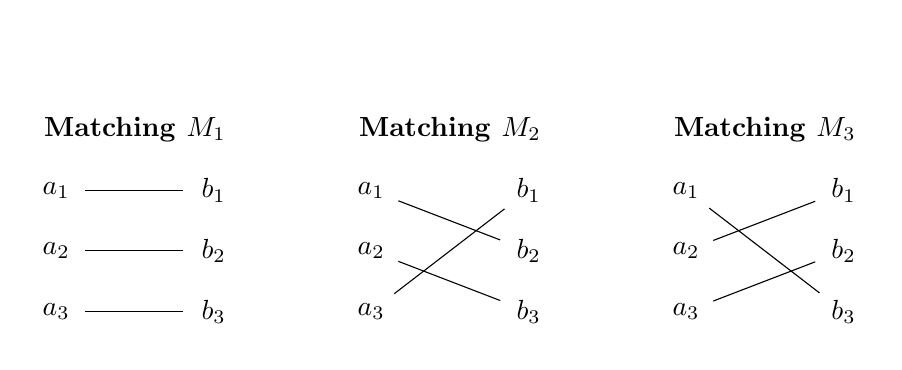
\begin{tikzpicture}[every node/.style={circle, draw=none}]
% Define the two sets of vertices
\node (A1) at (0,0/1.3) {$a_1$};
\node (A2) at (0,-1/1.3) {$a_2$};
\node (A3) at (0,-2/1.3) {$a_3$};
\node (B1) at (2,0/1.3) {$b_1$};
\node (B2) at (2,-1/1.3) {$b_2$};
\node (B3) at (2,-2/1.3) {$b_3$};

\node at (1,1/1.3) {\textbf{Matching }$M_1$};

\node (AA1) at (4,0/1.3) {$a_1$};
\node (AA2) at (4,-1/1.3) {$a_2$};
\node (AA3) at (4,-2/1.3) {$a_3$};
\node (BB1) at (6,0/1.3) {$b_1$};
\node (BB2) at (6,-1/1.3) {$b_2$};
\node (BB3) at (6,-2/1.3) {$b_3$};

\node at (5,1/1.3) {\textbf{Matching }$M_2$};

\node (AAA1) at (8,0/1.3) {$a_1$};
\node (AAA2) at (8,-1/1.3) {$a_2$};
\node (AAA3) at (8,-2/1.3) {$a_3$};
\node (BBB1) at (10,0/1.3) {$b_1$};
\node (BBB2) at (10,-1/1.3) {$b_2$};
\node (BBB3) at (10,-2/1.3) {$b_3$};

\node at (9,1/1.3) {\textbf{Matching }$M_3$};

% Draw edges between the two sets of vertices
\draw (A1) -- (B1);
\draw (AA1) -- (BB2);
\draw (AAA1) -- (BBB3);
\draw (AAA2) -- (BBB1);
\draw (A2) -- (B2);
\draw (AA2) -- (BB3);
\draw (AA3) -- (BB1);
\draw (AAA3) -- (BBB2);
\draw (A3) -- (B3);
\end{tikzpicture}
\end{center}

Here $M_1 \succ M_2$, $M_2 \succ M_3$, $M_3 \succ M_1$. Hence, no popular matching exists within the set $M_1, M_2, M_3$ as all of them lose an election.
\\

Hence we can ask the following question - what properties must a set of matchings $\mathcal{M}$ hold to guarantee the existence of popular matchings within the set $\mathcal{M}$. Before tackling this question we better equip ourself with the following definitions.

We define a \textit{Popularity Graph} for a given instance and set of matchings $\mathcal{M}$ to be a directed graph $G_{pop}$ where each vertex represents a matching in $\mathcal{M}$ and there is an edge from vertex $M$ to vertex $N$ if $N$ is more popular than $M$. It is obvious that a matching $M$ is popular if and only if it has no out-going edges in the Popularity Graph. It is easy to observe that there is no popular matching within a set of matchings if every vertex in the corresponding popularity graph is part of a cycle. 

Here, we ask the weaker question - which instances have no cycles in their corresponding popularity graphs and which do? Does there exist a characterisation of instances whose popularity graphs contain cycles?

Note that if an instance admits no cycles in its corresponding popularity graph then any subset of matchings in $\mathcal{M}$ will contain a popular matching.

\paragraph{Our Contribution:}
% In this report we answer this question positively for the restricted case of $3 \times 3$ instances ($|A| = |B| = 3$) with strict and complete preference lists. 

In this report we characterize those $3 \times 3$ instances ($|X| = |Y| = 3$) with strict and complete preference lists, which admit a 3-cycle in their popularity graphs. Further we derive a combinatorial result for the total number of such instances and generalise some of the lemmas to the $n \times n$ case.

\subsection{Stable matchings in instances with one-sided ties}
Another interesting setting is the setting of bipartite graphs with preferences involving one-sided ties. i.e. $G = (A \cup B, E)$ is a bipartite graph where each vertex in $A$ ranks its neighbours strictly and the preferences of the $B$ side allows ties. We can define stability in this case similar to the strict preference case, i.e. a \textit{weakly stable matching} is a matching with no blocking pairs where a blocking pair is defined as a pair of vertices $(a, b)$ such that $a \in A$, $b \in B$ and both $a$ and $b$ strictly prefer each other to their current matched partner.  We will use weak stability and stability analogously for the rest of this report. The Gale-Shapley algorithm can be generalised to output stable matchings in the case when the preference lists contain ties by simply breaking ties arbitrarily.

Similarly we can also define popular matchings in the same way as before, i.e. a matching $M$ is popular if there is no matching $N$ which is more popular than $M$. 

There are a several challenges that arise in the setting with ties as compared to the setting with strict preference lists. For instance, stable matchings need not be popular in this setting, neither do all stable matchings necessarily have the same size, in fact it is NP-hard to determine the existence of popular matchings in a given instance \cite{biro2010popular, cseh2017popular} as well as to compute a maximum or minimum size stable matching \cite{iwama2002stable, manlove2002hard}. 

\begin{center}
\textbf{Preferences:} \\
$a_1: \; b_2, \; b_1$ \; \; \; $b_1: \; (a_1)\phantom{ \; a_2}$ \\
$a_2: \; b_2\phantom{, \; b_1}$ \; \; \; $b_2: \; (a_1 \; a_2)$ \\
\end{center}

\begin{center}
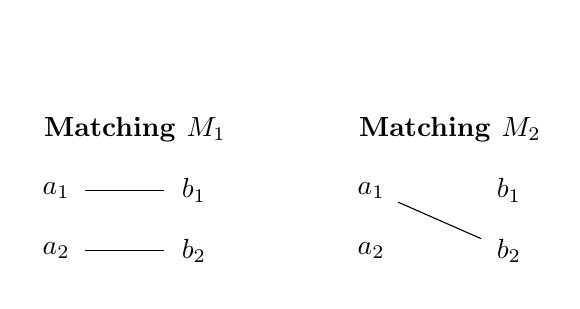
\begin{tikzpicture}[every node/.style={circle, draw=none}]
% Define the two sets of vertices
\node (A1) at (0,0/1.3) {$a_1$};
\node (A2) at (0,-1/1.3) {$a_2$};
\node (B1) at (1.75,0/1.3) {$b_1$};
\node (B2) at (1.75,-1/1.3) {$b_2$};

\node at (1,1/1.3) {\textbf{Matching }$M_1$};

\node (AA1) at (4,0/1.3) {$a_1$};
\node (AA2) at (4,-1/1.3) {$a_2$};
\node (BB1) at (5.75,0/1.3) {$b_1$};
\node (BB2) at (5.75,-1/1.3) {$b_2$};

\node at (5,1/1.3) {\textbf{Matching }$M_2$};

% Draw edges between the two sets of vertices
\draw (A1) -- (B1);
\draw (A2) -- (B2);
\draw (AA1) -- (BB2);
% \draw (AA2) -- (BB1);
\end{tikzpicture}
\end{center}

In the above example, both $M_1$ and $M_2$ are stable matchings with different sizes, also $M_1$ is more popular than $M_2$, hence $M_2$ is a stable matching which is not popular.

However there is a lot of work done on finding good approximation algorithms for computing large size stable matchings in the literature. We know of a $\frac{2}{3}$-approximation algorithm for finding a maximum size stable matching given by Zoltán Király \cite{kiraly2011better}. This was improved by Kavitha and Huang who gave a $\frac{15}{22}$-approximation algorithm \cite{huang2015improved}, though a more careful analysis of their algorithm by Felix Baukholt \textit{et al.} showed that Kavitha's algorithm is actually a $\frac{9}{13}$-approximation algorithm \cite{bauckholt2018approximability}. The best known approximation algorithm to date was given by Chi-Kit Lam \textit{et al.} which is a $\frac{e}{1 + e}$-approximation algorithm \cite{lam20191+}.

Since it is NP-hard to compute popular matchings we relax the notion of popularity to that of an \textit{unpopularity factor} as follows -

\begin{definition}
    A matching $M$ has unpopularity factor $u(M) = max_N(\lambda(M, N))$ where $\lambda(M, N)$ is defined as follows - 
    \begin{equation}
        \lambda(M, N) =
        \begin{cases}
            \frac{\phi(N, M)}{\phi(M, N)} & \text{if $\phi(M, N) \neq 0$} \\
            1 & \text{if $\phi(M, N) = 0$ and $\phi(N, M) = 0$} \\
            \infty & \text{otherwise}
        \end{cases}
    \end{equation}
\end{definition}

Hence, we now shift our goal from finding popular matchings to finding low unpopularity matchings. The only work known to us in this area is a recent work by Kavitha published in FSTTCS 2022 where she gives a proposal based algorithm to find a stable matching with unpopularity factor bounded by the longest tie length in the $B$ preferences \cite{kavitha2022stable}.

\paragraph{Our Contribution:}
We discuss algorithms that output large size stable matchings as well as algorithms that output low unpopularity stable matchings that were studied in the literature. We then talk about an algorithm that combines these two notions and gives matchings with both bounded unpopularity and large size. We also give a tight example for this bound. Finally we give a theoretical limit to how large the matchings with low unpopularity can be.

\section{Cycles in Popularity Graphs in the SM instance}
We will consider a restricted version of the \textit{Stable Marriage} or \textit{SM} instance in this section. More formally, an instance comprises of a graph $G = (X \cup Y, E)$ with $|X| = |Y| = n$ where each vertex $x \in X$ strictly ranks each vertex in $Y$ and vice-versa. We will call such an instance an $n \times n$ instance. It can be seen that all maximal matchings in such an instance will also be of maximum size. We will restrict our view to this set of matchings for the remainder of this section. 

\subsection{Redefining the ``more popular than" relation in a new light}
We say a vertex $v$ is \textit{promoted} from matching $M$ to $N$ if $v$ prefers $N$ over $M$. Similarly, we say a vertex $v$ is \textit{demoted} from matching $M$ to $N$ if $v$ prefers $M$ over $N$.

We can view the votes obtained in an election between two matchings $M$ and $N$ in terms of the number of vertices promoted and demoted in the transition from matching $M$ to $N$. Let us define the following 3 functions from the set $\mathcal{M} \times \mathcal{M}$ to $\mathbb{Z}$, where $\mathcal{M}$ is the set of maximal matchings in the given instance - 
\begin{enumerate}
    \item $p_x(M, N)$ is the number of vertices $x \in X$ that are promoted from $M$ to $N$.
    \item $d_x(M, N)$ is the number of vertices $x \in X$ that are demoted from $M$ to $N$.
    \item $t_x(M, N)$ is the number of vertices $x \in X$ that are indifferent from $M$ to $N$.
\end{enumerate}

Similarly, we define 
\begin{enumerate}
    \item $p_y(M, N)$ is the number of vertices $y \in Y$ that are promoted from $M$ to $N$.
    \item $d_y(M, N)$ is the number of vertices $y \in Y$ that are demoted from $M$ to $N$.
    \item $t_y(M, N)$ is the number of vertices $y \in Y$ that are indifferent from $M$ to $N$.
\end{enumerate}

We also define 
\begin{enumerate}
    \item $p(M, N) = p_x(M, N) + p_y(M, N)$ is the number of vertices $v \in X \cup Y$ that are promoted from $M$ to $N$.
    \item $d(M, N) = d_x(M, N) + d_y(M, N)$ is the number of vertices $v \in X \cup Y$ that are demoted from $M$ to $N$.
    \item $t(M, N) = t_x(M, N) + t_y(M, N)$ is the number of vertices $v \in X \cup Y$ that are indifferent from $M$ to $N$.
\end{enumerate}

We now use the above functions to redefine the ``more popular than" relation as follows.

\begin{lemma}
    A matching $N$ is more popular than a matching $M$ if and only if $p(M, N) > d(M, N)$
\end{lemma}

It can be easily observed that since each vertex $x \in X$ is either promoted, demoted or indifferent from $M$ to $N$, $p_x(M, N) + d_x(M, N) + t_x(M, N) = n$. Similarly since each vertex $y \in Y$ is either promoted, demoted or indifferent from $M$ to $N$, $p_y(M, N) + d_y(M, N) + t_y(M, N) = n$. Hence we have the following relation -
\begin{lemma}
    $p(M, N) + d(M, N) + t(M, N) = 2n$
\end{lemma}

We also have the following property for indifference when transitioning from a perfect matching $M$ to another perfect matching $N$, $t_x(M, N) = t_y(M, N)$ and hence $t(M, N)$ must be even. This is obvious from the fact that no vertices are unmatched in $M$ or $N$ and for every vertex $x$ that remains indifferent, its corresponding matched partner also remains indifferent in the transition.

% \begin{proof}
%     For each $x \in X$ that remains indifferent from $M$ to $N$, its corresponding partner $y \in Y$ would also remain indifferent in the transition $M \rightarrow N$.
% \end{proof}

\subsection{Characterising the $3 \times 3$ case}
Consider a $3 \times 3$ instance $G = (X \cup Y, E)$ where $X = \{x_1, x_2, x_3\}$ and $Y = \{y_1, y_2, y_3\}$ and $E = \{(x, y): x \in X \land y \in Y\}$. Let the set of maximal matchings in this instance be denoted by $\mathcal{M}$. In this section we wish to characterise instances that contain 3-cycles in the popularity graph. Consider 3 matchings $M_1$, $M_2$ and $M_3$ that form a 3-cycle in the popularity graph $G_{pop}$, that is $M_1 \prec M_2$, $M_2 \prec M_3$ and $M_3 \prec M_1$. Throughout the remainder of this section we will assume a $3 \times 3$ instance as described above.

% We first prove that all cycles in the graph $G_{pop}$ have size $= 3$

% \begin{lemma}
%     All cycles in the graph $G_{pop}$ have size 3
% \end{lemma}

% \begin{proof}
%     Obviously a cycle cannot have size $2$ as that would mean that there exists matchings $M_1$ and $M_2$ such that $M_1 \succ M_2$ and $M_2 \succ M_1$ which is not possible.

%     Let there exists a cycle $M_1, M_2, ..., M_k$ of size $k \geq 4$
% \end{proof}

\begin{lemma}
$M_1 \cap M_2 \cap M_3 = \phi$, i.e. no edge appears in all 3 matchings.
\end{lemma}

\begin{proof}
Without loss of generality, let us assume $(x_1, y_1)$ edge exists in all 3 matchings. This leaves only 2 possible maximal matchings with the edge $(x_1, y_1)$, i.e. $\{(x_1, y_1), (x_2, y_2), (x_3, y_3)\}$ and $\{(x_1, y_1), (x_2, y_3), (x_3, y_2)\}$, hence there cannot be 3 distinct matchings with the edge $(x_1, y_1)$.
\end{proof}

\begin{lemma}
Every vertex must be demoted at least once in the sequence of transitions $M_1 \rightarrow M_2 \rightarrow M_3 \rightarrow M_1$.
\end{lemma}

\begin{proof}
If a vertex $x$ is never demoted then in each transition it is either promoted or remains indifferent. But from Lemma 2.3 $x$ cannot remain indifferent in all 3 transitions as then the edge between $x$ and its matched partner will appear in all 3 matchings. Hence $x$ must have been promoted at least once. Let $x$ be matched with $\alpha_1$, $\alpha_2$, $\alpha_3$ in $M_1$, $M_2$, $M_3$ respectively where $\alpha_i$'s need not be distinct. Since in each transition $x$ is either promoted or remains indifferent and $x$ cannot be indifferent in all 3 transitions, hence $\alpha_3$ must be preferred over $\alpha_1$ in the preference list of $x$, as if not then $x$ would be indifferent in the transition $M_1 \rightarrow M_2$ and $M_2 \rightarrow M_3$ and hence $\alpha_1, \alpha_2, \alpha_3$ would all be the same vertex. But then $x$ is demoted in the transition $M_3 \rightarrow M_1$, hence a contradiction to the fact that $x$ was never demoted. 
\end{proof}

\begin{lemma}
    The sum of number of demotions in all transitions in a 3-cycle $\geq 6$
\end{lemma}

\begin{proof}
        From Lemma 2.4, each vertex is demoted at least once, and there are 6 such vertices, hence the total number of demotions $\geq 6$
\end{proof}

\begin{lemma}
    The number of demotions in each transition in a 3-cycle $ \leq 2$
\end{lemma}

\begin{proof}
    Let $M_i \rightarrow M_j$ be a transition in the 3-cycle and $d(M_i, M_j) \geq 3$ then $p(M_i, M_j) = 6 - d(M_i, M_j) - t(M_i, M_j) \leq 3$. But this is a contradiction as $p(M_i, M_j) > d(M_i, M_j)$.
\end{proof}

\begin{lemma}
    In each transition in a 3-cycle, the total number of promotions is exactly 4, demotions is exactly 2 and indifference is 0.
\end{lemma}

\begin{proof}
    From Lemma 2.5 we have $d(M_1, M_2) + d(M_2, M_3) + d(M_3, M_1) \geq 6$, from Lemma 2.6 we have $d(M_1, M_2) + d(M_2, M_3) + d(M_3, M_1) \leq 6$.  Hence $d(M_1, M_2) + d(M_2, M_3) + d(M_3, M_1) = 6$ and $d(M_1, M_2) = d(M_2, M_3) = d(M_3, M_1) = 2$. Also since for each transition $M_i \rightarrow M_j$ in the 3-cycle $t(M_i, M_j)$ is even $\implies$ $t(M_i, M_j) = 0$ as if $t(M_i, M_j) \geq 2$ then $p(M_i, M_j) \leq 2$ which is a contradiction since $p(M_i, M_j) > d(M_i, M_j)$.
\end{proof}

Since from the above Lemma, the indifference in each transition is 0, this immediately implies the following Corollary.

\begin{corollary}
$M_1, M_2, M_3$ are pairwise disjoint.
\end{corollary}

We now define functions $\ell$ and $r$ which will be useful for us to ``rotate" along the preferences from one matching to another. This will be useful when proving relationships between the matchings that participate in a cycle in the popularity graph -
\begin{itemize}
    \item $\ell(u, v)$ denotes the vertex which $u$ prefers by exactly one rank to $v$, except when $v$ is the top choice in which case it denotes the last choice of $u$.
    \item $r(u, v)$ denotes the vertex $v'$ such that $\ell(u, v')$ is $v$.
\end{itemize}

Intuitively, $\ell$ and $r$ represent the left and right position of $v$ in the preference list of $u$ in a cyclic fashion where preference lists are ordered from left (best choice) to right (worst choice).

We say a permutation $P_1$ of $n$ elements is a cyclic permutation of another permutation $P_2$ of $n$ elements if $\exists i$ such that the $\forall 0 \leq j \leq n$, the following equation holds-

\begin{equation}
    \text{$j^{th}$ element of $P_1$} =
    \begin{cases}
        \text{$(i+j)^{th}$ element of $P_2$} & \text{if $i + j \leq n$} \\
        \text{$(i+j-n)^{th}$ element of $P_2$} & \text{if $i + j > n$} \\
    \end{cases}
\end{equation}

We define the notion of an \textit{X-cyclic} and \textit{Y-cyclic} instance as follows - 
\begin{definition}
    An instance is said to be X-cyclic if the preference lists of all vertices $x \in X$ are cyclic permutations of each other.
\end{definition}

\begin{definition}
    An instance is said to be Y-cyclic if the preference lists of all vertices $y \in Y$ are cyclic permutations of each other.
\end{definition}
    
It is easy to see that $\ell(x, y)$ and $r(x, y)$ are invariant of $x \in X$ for X-cyclic permutations. In these contexts we will simply write it as $\ell(y)$ and $r(y)$, similarly for Y-cyclic permutations we will simply write $\ell(y, x)$ and $r(y, x)$ as $\ell(x)$ and $r(x)$ respectively.

It is also easy to see that the function $\ell$ is one-to-one when we have X-cyclicity. i.e. $x_1 \neq x_2 \implies \ell(x_1) \neq \ell(x_2)$. From this we can conveniently define a notion of transforming one matching to another by promoting all $x$ vertices not matched to its top choice by one rank and demoting any $x$ matched to its top choice to its last choice. Hence we define $LS_X(M)$ (LS stands for left-shift) for X-cyclic instances as the matching obtained by replacing every $(x, y)$ edge in the matching with an $(x, \ell(y))$ edge. We define $LS_Y(M)$ for a Y-cyclic instance in a similar fashion.

\begin{lemma}
    In each of the transitions $M_i$ to $M_j$ in the 3-cycle, every vertex gets promoted by exactly one rank, except when it is matched to its top choice in which case it gets demoted to its least favourable choice. In other words $M_j = LS_X(M_i) = LS_Y(M_i)$
\end{lemma}

\begin{proof}
    Consider the matched partners of some vertex $x \in X$ in $M_1, M_2, M_3$. Since all these matchings are pairwise disjoint, the matched partners of $x$ in all 3 matchings are distinct, let them be $y_1, y_2, y_3$ respectively. Now we either have $y_1 = r(x, y_3)$, $y_2 = r(x, y_1)$, $y_3 = r(x, y_2)$ or $y_1 = \ell(x, y_3)$, $y_2 = \ell(x, y_1)$, $y_3 = \ell(x, y_2)$. Since sum of number of demotions in each transition is exactly 6 and each of the 6 vertices gets demoted at least once $\implies$ each vertex gets demoted exactly once. Hence, we can rule out the former case as if it were true then the total number of times $x$ is demoted in all 3 transitions is 2 which is a contradiction. Hence $y_1 = \ell(x, y_3)$, $y_2 = \ell(x, y_1)$, $y_3 = \ell(x, y_2)$. The similar proof holds for the $Y$ side.
\end{proof}

\begin{lemma}
    If an instance admits a 3-cycle in the popularity graph then the instance must be both X-cyclic and Y-cyclic
\end{lemma}

\begin{proof}
    Let $M_i \rightarrow M_j$ be one of the transitions in the 3-cycle. We know from the Lemma 2.9 that $M_j = LS_X(M_i) = LS_Y(M_i)$. Now assume without loss of generality that the preference of $x_1$ and $x_2$ are cyclic permutations of $y_1, y_2, y_3$ in that order and the preference of $x_3$ is a cyclic permutation of $y_3, y_2, y_1$. This assumption is justified because of the fact every preference list for a vertex in $X$ can only be of these two forms. Also let us assume without loss of generality that $x_1$ is matched to $y_1$ in $M_i$. We have the following two cases
    \begin{itemize}
        \item Case-1: $x_2$ is matched to $y_2$ and $x_3$ to $y_3$ in $M_i$ \\
        On left shifting we can conclude that both $x_2$ and $x_3$ would be matched to $y_1$ in $M_j$ which is not possible.
        \item Case-2: $x_2$ is matched to $y_3$ and $x_3$ to $y_2$ in $M_i$ \\
        On left shifting we can conclude that both $x_1$ and $x_3$ would be matched to $y_3$ in $M_j$ which is not possible.
    \end{itemize}
\end{proof}

Now we show a sufficient and necessary condition for when an instance which is both X-cyclic and Y-cyclic satisfies the property $LS_X(M) = LS_Y(M)$ for some maximal matching $M$.

We first define \textit{niceness} of a matching as follows-
\begin{definition}
    A matching $M$ is nice if $\forall x \in X, y \in Y, (x, y) \in M \implies (\ell(x), r(y)) \in M$
\end{definition}

\begin{lemma}
    Let the instance $I$ be both, an X-cyclic and Y-cyclic instance, then $LS_X(M) = LS_Y(M)$ if and only if $M$ is nice
\end{lemma}

\begin{proof}
    Lets call $LS_X(M)$ as $M_X$ and $LS_Y(M)$ as $M_Y$
    We first prove the forward direction. Let $M_X = M_Y$ and $M$ is not nice, hence there must be an edge $(x, y) \in M$ such that $(\ell(x), r(y)) \notin M$. From the definition of $M_Y$, vertex $y$ is matched to $\ell(x)$ in $M_Y$. Now since $M_Y = M_X$, $\ell(x)$ is matched to $y$ in $M_X$, hence we can say that $\ell(x)$ must have been matched to $r(y)$ in $M$, hence a contradiction to the fact that $(\ell(x), r(y)) \notin M$.

    Now we prove the backward direction, assume that $M$ is nice, now we will explicitly construct $M_X$ and $M_Y$ and show that they are equal. Consider some $x \in X$, $y \in Y$ such that $(x, y)$ is in $M$. Since $M$ is nice, we can immediately claim that $(\ell(x), r(y))$ and $(\ell(\ell(x)), r(r(y))) = (r(x), \ell(y)) \in M$, hence we write the matching as $M = \{(x,y), (\ell(x), r(y)), (r(x), \ell(y))\}$. From this we construct 
    \\
    $M_X = \{(x, \ell(y)), (\ell(x), \ell(r(y))), (r(x), \ell(\ell((y))))\} \\ \phantom{M_X } = \{(x, \ell(y)), (\ell(x), y), (r(x), r(y))\}$
    \\
    Similarly we construct
    \\
    $M_Y = \{(\ell(x),y), (\ell(\ell(x)), r(y)), (\ell(r(x)), \ell(y))\} \\ \phantom{M_X } = \{(\ell(x), y), (r(x), r(y)), (x, \ell(y))\}$
    \\
    Hence $M_X = M_Y$
\end{proof}

Hence we have the final characterisation as follows -

\begin{theorem}
    An instance has a 3-cycle in the popularity graph if and only if the following conditions hold - 
    \begin{itemize}
        \item the preferences are both X-cyclic and Y-cyclic.
        \item $\exists$ a matching $M$ such that $M$ is nice and
        \item $M$ has exactly 2 vertices matched to its 1st preference, 2 vertices matched to its 2nd preference and 2 vertices matched to its 3rd preference.
    \end{itemize}
\end{theorem}

\begin{proof}
    We prove the forward direction first - Let the popularity graph $G_{pop}$ has a 3-cycle $M_1 \rightarrow M_2 \rightarrow M_3 \rightarrow M_1$. We already know from the Lemma 2.9 and 2.10 that the instance is both X-cyclic and Y-cyclic and each $M_i$ must be nice.
    We know from Lemma 2.7 that the transition from $M_1$ to $M_2$ must have exactly 2 demotions. Also since $M_2 = LS_X(M_1) = LS_Y(M_1)$, the two vertices that are demoted must be matched to their top preference (if not then it would be promoted from its $i^{th}$ ranked choice to its $i-1^{th}$ ranked choice in the transition from $M_1$ to $M_2$). Hence $M_1$ has exactly 2 vertices matched to their 1st preference. Now since $M_3 = LS_X(M_2) = LS_Y(M_2)$ and $M_1 = LS_X(M_3) = LS_Y(M_3)$, from a similar argument we can conclude that both $M_2$ and $M_3$ have exactly 2 vertices matched to their top choices. But each vertex matched to its 1st preference in $M_2$ must have been matched to their 2nd preference in $M_1$ since $M_2$ is formed by cyclically left-shifting each vertex by 1 on its preference list. Hence $M_1$ has exactly 2 vertices matched to their 2nd preference. Similarly each vertex that is matched to its 1st preference in $M_3$ must have been matched to its 3rd preference in $M_1$. Hence $M_1$ has exactly 2 vertices matched to their 3rd preference.

    Now assume that the instance is X-cyclic and Y-cyclic and there exists a matching $M$ with 2 vertices matched to their 1st, 2nd and 3rd preference. Let $a$ and $b$ be matched to their 1st preference in $M$, $c$ and $d$ to their 2nd, $e$ and $f$ to their 3rd. Let $M' = LS_X(M) = LS_Y(M)$. Then $a$ and $b$ would be demoted from their transition from $M$ to $M'$ and the rest of the vertices would be promoted, also $a$ and $b$ would be matched with their 3rd preference in $M'$, $c$ and $d$ to their 1st, and $e$ and $f$ to their 2nd. Similarly let $M'' = LS_X(M') = LS_Y(M')$. Then in the transition from $M'$ to $M''$, $c$ and $d$ would be demoted and the rest of the vertices would be promoted. Also $a$ and $b$ would be matched with their 2nd preference, $c$ and $d$ to their 3rd and $e$ and $f$ to their 1st in $M''$. Obviously $LS_X(M'') = LS_Y(M'') = M$ (left shifting $M$ 3 times would lead us back to $M$). On following a similar argument we can say that $e$ and $f$ are demoted in the transition from $M''$ to $M$ and the rest of the vertices are promoted. Hence we have found a 3-cycle $M \rightarrow M' \rightarrow M'' \rightarrow M$.
\end{proof}

\subsection{A combinatorial result on the number of instances that admit 3-cycles}
In this section, we use the characterization derived to prove that out of all the $(3!)^6 = 46656$ possible instances, exactly 360 of them admit 3-cycles in their corresponding popularity graph. Though this may seem like a small fraction (0.77\%), it turns out that the fraction increases very rapidly for the general $n \times n$ case and in most cases the number of instances that admit 3-cycles in its popularity graph is significantly larger than the instances without 3-cycles.

\begin{theorem}
    Out of $(3!)^6 = 46656$ possible instances $360$ of them have a 3-cycle in the popularity graph.
\end{theorem}

\begin{proof}
    Consider a $3 \times 3$ instance with a 3-cycle in the popularity graph. Let us temporarily forget about the preferences of the individual vertices and observe what the matching would look like in the preferences space (with the vertices in the preference replaced by blanks), consider the preferences below - \\ \\
    $x_1: \; \circled{\rule{0.3cm}{0.15mm}} \; \; \rule{0.3cm}{0.15mm} \; \; \rule{0.3cm}{0.15mm}$ \phantom{This text will be invisible} $y_1: \; \rule{0.3cm}{0.15mm} \; \; \rule{0.3cm}{0.15mm} \; \; \circled{\rule{0.3cm}{0.15mm}}$ \\
    $x_2: \; \circled{\rule{0.3cm}{0.15mm}} \; \; \rule{0.3cm}{0.15mm} \; \; \rule{0.3cm}{0.15mm}$ \phantom{This text will be invisible} $y_2: \; \rule{0.3cm}{0.15mm} \; \; \circled{\rule{0.3cm}{0.15mm}} \; \; \rule{0.3cm}{0.15mm}$ \\
    $x_3: \; \rule{0.3cm}{0.15mm} \; \; \circled{\rule{0.3cm}{0.15mm}} \; \; \rule{0.3cm}{0.15mm}$ \phantom{This text will be invisible} $y_3: \; \rule{0.3cm}{0.15mm} \; \; \rule{0.3cm}{0.15mm} \; \; \circled{\rule{0.3cm}{0.15mm}}$ \\

    Consider a matching formed by the circled blanks. Here the 3rd point in the Theorem 2.11 holds true and hence all that remains to produce an instance with a 3-cycle is to cleverly list the preferences so that the 1st and 2nd point of Theorem 2.11 also holds. Let there exists such a clever listing. Without loss of generality let $M$ in Theorem 2.12 be the matching that matched $x_1$ to its 1st preference, as if it doesn't then we can left-shift $M$ enough times to get such a matching that is still a valid $M$ for Theorem 2.11 and a given instance. Also let us call the above preferences diagram for the $x$ preferences an \textit{x-pattern} and similarly call the $y$ preferences in the above diagram a \textit{y-pattern}. Also if an x-pattern and y-pattern satisfy the 3rd criteria of Theorem 2.11 then we call the patterns are compatible. Now we break the proof into two parts.
    \\ \\
    Let us fix the pattern such that the 3rd criteria of Theorem 2.11 is satisfied. We can then choose to fill the circled blank in the $x_1$ preference in 3 ways (either $y_1$, $y_2$ or $y_3$), we can then fill the circled blanks in $x_2$ preference in 2 ways (either of the remaining unchosen $y$'s), and are left with only 1 way to fill the circled blank in $x_3$'s preference. Observe that fixing the values of the circled blanks in the $x$ preferences automatically fixes the circled blanks in the $y$ preferences and there are $3 \times 2 \times 1 = 6$ ways to do so. Now we can fix the $x$ preferences to satisfy condition 1 of Theorem 2.12 by specifying whether the $x$ preferences are cyclic permutations of $(y_1, y_2, y_3)$ or $(y_3, y_2, y_1)$ (we only have these 2 cases) and hence we can do this in 2 ways. After fixing this we can accordingly fix the $y$ preferences so that $LS_X(M) = LS_Y(M)$ and hence $M$ is nice in the generated instance. Hence there are $6 \times 2 = 12$ such instances for a given compatible x-pattern and y-pattern.
    \\ \\
    Now we can count the number of compatible $x$ and $y$ patterns by listing all the possible $x$ patterns that match $x_1$ to its top choice and counting the number of $y$ patterns that are compatible to it. We have the following cases -
    \begin{itemize}
        \item 
        $x_1: \; \circled{\rule{0.3cm}{0.15mm}} \; \; \rule{0.3cm}{0.15mm} \; \; \rule{0.3cm}{0.15mm}$ \\
        $x_2: \; \rule{0.3cm}{0.15mm} \; \; \circled{\rule{0.3cm}{0.15mm}} \; \; \rule{0.3cm}{0.15mm}$ \\
        $x_3: \; \rule{0.3cm}{0.15mm} \; \; \rule{0.3cm}{0.15mm} \; \; \circled{\rule{0.3cm}{0.15mm}}$ \\
        Here we choose a $y$ to match to its 1st choice in 3 ways, we then choose one of the remaining two $y$'s to match to its 2nd choice in 2 ways and match the last $y$ to its 3rd choice. We do this in $3 \times 2 \times 1 = 6$ ways.
        \item 
        $x_1: \; \circled{\rule{0.3cm}{0.15mm}} \; \; \rule{0.3cm}{0.15mm} \; \; \rule{0.3cm}{0.15mm}$ \\
        $x_2: \; \rule{0.3cm}{0.15mm} \; \; \rule{0.3cm}{0.15mm} \; \; \circled{\rule{0.3cm}{0.15mm}}$ \\
        $x_3: \; \rule{0.3cm}{0.15mm} \; \; \circled{\rule{0.3cm}{0.15mm}} \; \; \rule{0.3cm}{0.15mm}$ \\
        Here we choose a $y$ to match to its 1st choice in 3 ways, we then choose one of the remaining two $y$'s to match to its 2nd choice in 2 ways and match the last $y$ to its 3rd choice. We do this in $3 \times 2 \times 1 = 6$ ways.
        \item 
        $x_1: \; \circled{\rule{0.3cm}{0.15mm}} \; \; \rule{0.3cm}{0.15mm} \; \; \rule{0.3cm}{0.15mm}$ \\
        $x_2: \; \circled{\rule{0.3cm}{0.15mm}} \; \; \rule{0.3cm}{0.15mm} \; \; \rule{0.3cm}{0.15mm}$ \\
        $x_3: \; \rule{0.3cm}{0.15mm} \; \; \circled{\rule{0.3cm}{0.15mm}} \; \; \rule{0.3cm}{0.15mm}$ \\
        Here we choose two $y$'s and match them to their 3rd choice and match the leftover $y$ to its 2nd choice in $^3C_2 = 3$ ways
        \item 
        $x_1: \; \circled{\rule{0.3cm}{0.15mm}} \; \; \rule{0.3cm}{0.15mm} \; \; \rule{0.3cm}{0.15mm}$ \\
        $x_2: \; \circled{\rule{0.3cm}{0.15mm}} \; \; \rule{0.3cm}{0.15mm} \; \; \rule{0.3cm}{0.15mm}$ \\
        $x_3: \; \rule{0.3cm}{0.15mm} \; \; \rule{0.3cm}{0.15mm} \; \; \circled{\rule{0.3cm}{0.15mm}}$ \\
        Here we choose two $y$'s and match them to their 2nd choice and match the leftover $y$ to its 3rd choice in $^3C_2 = 3$ ways
        \item 
        $x_1: \; \circled{\rule{0.3cm}{0.15mm}} \; \; \rule{0.3cm}{0.15mm} \; \; \rule{0.3cm}{0.15mm}$ \\
        $x_2: \; \rule{0.3cm}{0.15mm} \; \; \circled{\rule{0.3cm}{0.15mm}} \; \; \rule{0.3cm}{0.15mm}$ \\
        $x_3: \; \circled{\rule{0.3cm}{0.15mm}} \; \; \rule{0.3cm}{0.15mm} \; \; \rule{0.3cm}{0.15mm}$ \\
        Here we choose two $y$'s and match them to their 3rd choice and match the leftover $y$ to its 2nd choice in $^3C_2 = 3$ ways
        \item 
        $x_1: \; \circled{\rule{0.3cm}{0.15mm}} \; \; \rule{0.3cm}{0.15mm} \; \; \rule{0.3cm}{0.15mm}$ \\
        $x_2: \; \rule{0.3cm}{0.15mm} \; \; \rule{0.3cm}{0.15mm} \; \; \circled{\rule{0.3cm}{0.15mm}}$ \\
        $x_3: \; \circled{\rule{0.3cm}{0.15mm}} \; \; \rule{0.3cm}{0.15mm} \; \; \rule{0.3cm}{0.15mm}$ \\
        Here we choose two $y$'s and match them to their 2nd choice and match the leftover $y$ to its 3rd choice in $^3C_2 = 3$ ways
        \item 
        $x_1: \; \circled{\rule{0.3cm}{0.15mm}} \; \; \rule{0.3cm}{0.15mm} \; \; \rule{0.3cm}{0.15mm}$ \\
        $x_2: \; \rule{0.3cm}{0.15mm} \; \; \circled{\rule{0.3cm}{0.15mm}} \; \; \rule{0.3cm}{0.15mm}$ \\
        $x_3: \; \rule{0.3cm}{0.15mm} \; \; \circled{\rule{0.3cm}{0.15mm}} \; \; \rule{0.3cm}{0.15mm}$ \\
        Here we choose two $y$'s and match them to their 3rd choice and match the leftover $y$ to its 1st choice in $^3C_2 = 3$ ways
        \item 
        $x_1: \; \circled{\rule{0.3cm}{0.15mm}} \; \; \rule{0.3cm}{0.15mm} \; \; \rule{0.3cm}{0.15mm}$ \\
        $x_2: \; \rule{0.3cm}{0.15mm} \; \; \rule{0.3cm}{0.15mm} \; \; \circled{\rule{0.3cm}{0.15mm}}$ \\
        $x_3: \; \rule{0.3cm}{0.15mm} \; \; \rule{0.3cm}{0.15mm} \; \; \circled{\rule{0.3cm}{0.15mm}}$ \\
        Here we choose two $y$'s and match them to their 2nd choice and match the leftover $y$ to its 1st choice in $^3C_2 = 3$ ways
    \end{itemize}

    Hence the total number of compatible patterns is $6 + 6 + 3 + 3 + 3 + 3 + 3 + 3 = 30$. The total number of instances that admit a 3-cycle would thus be $30 \times 12 = 360$
\end{proof}

\subsection{Some generalisations to the $n \times n$ case}
In this section, we aim to generalize some of the lemmas discussed in section 2.2 for a k-cycle in the popularity graph in the $n \times n$ instance.

Consider an $n \times n$ instance $G = (X \cup Y, E)$ where $X = \{x_1, x_2, ..., x_n\}$ and $Y = \{y_1, y_2, ..., y_n\}$ and $E = \{(x, y): x \in X \land y \in Y\}$. Let the set of maximal matchings in this instance be denoted by $\mathcal{M}$. Consider $k$ matchings $M_1, M_2, ..., M_k$ that form a $k$-cycle in the popularity graph $G_{pop}$, that is $M_1 \prec M_2$, $M_2 \prec M_3$ ... $M_{k-1} \prec M_k$, $M_k \prec M_1$.

Let us assume that $M_1 \cap M_2 \cap ... \cap M_k = \phi$, as if not then the problem effectively reduces to the $(n - 1) \times (n - 1)$ case.

\begin{lemma}
Each vertex must be demoted at least once in the sequence of transitions $M_1 \rightarrow M_2 \rightarrow ... \rightarrow M_k \rightarrow M_1$.
\end{lemma}

\begin{proof}
Similar to the $3 \times 3$ case.
\end{proof}

\begin{lemma}
    The sum of demotions in each transition in a $k$-cycle $\geq 2n$
\end{lemma}

\begin{proof}
    From Lemma 2.13, each vertex is demoted at least once, and there are $2n$ such vertices, hence the total number of demotions $\geq 2n$
\end{proof}

\begin{lemma}
    The number of demotions in each transition in a $k$-cycle $ \leq n-1$
\end{lemma}

\begin{proof}
    Let the number of demotions in the transition $M_i \rightarrow M_j$ in the $k$-cycle be $\geq n$, hence from $p(M_i, M_j) + d(M_i, M_j) + t(M_i, M_j) = 2n$, we have $p(M_i, M_j) = 2n - d(M_i, M_j) - t(M_i, M_j) \leq 2n - d(M_i, M_j) \leq n$, hence we have $p(M_i, M_j) \leq d(M_i, M_j)$ which is a contradiction as $M_j$ is more popular than $M_i$.
\end{proof}

\begin{theorem}
    The total sum of indifferences of all transition $\leq 2nk - 4n - 2k$
\end{theorem}

\begin{proof}
    For each transition $M_i, M_j$ in the $k$-cycle we have $p(M_i, M_j) > d(M_i, M_j)$. Also $p(M_i, M_j) + d(M_i, M_j) = 2n - t(M_i, M_j) = even$, hence $p(M_i, M_j) - d(M_i, M_j)$ must be even $\implies p(M_i, M_j) \geq d(M_i, M_j) + 2$, hence from Lemma 2.15 we have $\sum p(M_i, M_j) \geq 2n + 2k$ and $\sum d(M_1, M_2) \geq 2n$, we also have $\sum (p(M_1, M_2) + d(M_1, M_2) + t(M_1, M_2)) = 2nk \ \implies \sum t(M_1, M_2) \leq 2nk - 4n - 2k$
\end{proof}

Note that plugging values $n = k = 3$ in the above formula gives us the total sum of indifferences to be $0$ which is evident from the previous sections. However it is the non-zero indifference in the general case that makes generalising to the $n \times n$ case tougher than the restriced $3 \times 3$ case as each transition can have a range of $p$, $d$ and $t$ values as opposed to the 3-cycles in $3 \times 3$ case where each $p$, $d$, $t$ take values 4, 2 and 0 respectively.

\section{Low unpopularity stable matchings with one-sided ties}
In this section we discuss popularity and size of stable matchings in bipartite graphs with preferences and one-sided ties. Our instance consists of a bipartite graph $G = (A \cup B, E)$ where each vertex in the $A$ side has a strict preference list ranking its neighbours and each vertex in $B$ has a preference list that may contain ties in its rankings. Our specific interest lies in finding large size stable matchings with low unpopularity factor in the given instance.

\subsection{Large size stable matchings}
The problem of finding large size stable matchings in the given setting has been studied extensively, here we will mainly refer to the simple algorithm given by Király\cite{kiraly2011better}. This is a proposal based algorithm similar to the well known Gale-Shapley algorithm where the $A$ side proposes and the $B$ side that admits ties in its preferences disposes. The algorithm maintains a level/status of 1 or 2 for each vertex in $A$. A vertex $a \in A$ gets promoted from level-1 to level-2 after a proposer has been rejected at least once by all vertices in $B$ as a level-1 vertex. This level-2 vertex will then be preferred over all level-1 vertices that it is tied to in the $B$ preferences. The algorithm is given at the start of the next page.

% \begin{algorithm}
% \caption{Gale-Shapley Algorithm}\label{alg:gale-shapley}
% \begin{algorithmic}[1]

% \Procedure{GaleShapley}{$M, W$}
% \State Initialize all $m\in M$ and $w\in W$ to be free
% \While{there exists a free man $m$}
% \State Choose a free man $m$
% \State Let $w$ be the highest-ranked woman in $m$'s preference list to whom $m$ has not yet proposed
% \If{$w$ is free}
% \State $(m, w)$ become engaged
% \Else
% \State Let $m'$ be the man whom $w$ is currently engaged to
% \If{$w$ prefers $m$ to $m'$}
% \State $(m, w)$ become engaged, $m'$ becomes free
% \Else
% \State $m$ remains free
% \EndIf
% \EndIf
% \EndWhile
% \EndProcedure

% \end{algorithmic}
% \end{algorithm}

\begin{algorithm}
\caption{Király's Algorithm}\label{alg:gale-shapley}
\begin{algorithmic}[1]

\Procedure{Király}{$A, B$}
\State Initialize all $a\in A$ and $b\in B$ to be free
\State Initialize all $a\in A$ to level-1
\While{there exists a free vertex $a \in A$}
\State Choose a free vertex $a \in A$
\State Let $b$ be the most preferred vertex in $a$'s preference list to who $a$ has not yet proposed with its current status
\If{$b$ is free}
\State $(a, b)$ become engaged
\Else
\State Let $a'$ be the current matched partner of $b$
\If{$b$ prefers $a$ to $a'$}
\State $(a, b)$ become engaged, $a'$ becomes free
\ElsIf{$b$ is indifferent between $a$ and $a'$}
\If{$a$ is level-2 and $a'$ is level-1}
\State $(a, b)$ become engaged, $a'$ becomes free
\EndIf
\Else
\State $a$ remains free
\If{$a$ has exhausted its prefernce list and is level-1}
\State $a$ is promoted to level-2
\EndIf
\EndIf
\EndIf
\EndWhile
\EndProcedure

\end{algorithmic}
\end{algorithm}

The above algorithm computes a stable matching with size approximation $\frac{2}{3}$ to the maximum size stable matching, i.e. $|M_{alg}| \geq \frac{2}{3}|M_{opt}|$ where $M_{opt}$ is the maximum size stable matching and $M_{alg}$ is the matching obtained by our algorithm. 

Note how in this algorithm every $b \in B$ that gets matched at some point in the algorithm remains matched for the remainder of the algorithm and never becomes free, in fact the matched partner of $b$ never gets worse as the only time $b$ rejects a proposal is for a vertex thats either better or equal in rank to the rejected vertex. This justifies stability.

Király proves the size bound of $\frac{2}{3}$ by showing that $M \oplus M_{opt}$ has no length 3 augmenting paths \cite{kiraly2011better}.

\begin{theorem}
    $M \oplus M_{opt}$ has no length 3 augmenting path
\end{theorem}

\begin{proof}
    Let the path $\{(a', b), (b, a), (a, b')\}$ be a length 3 augmenting path, i.e. $(a, b) \in M$ and $(a', b) \in M_{opt}$, $(a, b') \in M_{opt}$. Since $b'$ is unmatched in $M$, it must be the case that it never got a proposal. Hence $a$ must be a level-1 vertex as if it were level-2 then it would have proposed to $b'$ at some point and got rejected. Further, $a$ must prefer $b$ over $b'$ or else it would've proposed to $b'$ before $b$. Also, since $a'$ is unmatched in $M$, it must be a level-2 vertex that exhausted its list. Hence it must have proposed to $b'$ with level-2 status at some point in the algorithm. But $b'$ is finally matched to $a$ which is at level-1 at the end of the algorithm. Hence it cannot be the case that $b$ prefers $a'$ over $a$ , neither can it be indifferent between $a'$ and $a$ as in both cases its neighbourhood worsens, so $b$ must prefer $a$ over $a'$. Hence, $(a, b)$ is a blocking pair in $M_{opt}$ contradicting the stability of $M_{opt}$.
\end{proof}

\subsubsection{Király's reduction}
It has been shown in \cite{cseh2018popular} that Király's algorithm can also be simulated by applying the well known Gale-Shapley algorithm on a cleverly constucted reduced instance for the original instance, we will call this reduction \textit{Király's Reduction}. The reduction is as follows -
\begin{enumerate}
    \item $\forall a \in A$ add $a^*$ to the set $A$ and $a$'s last resort vertex $l(a)$ to the set $B$
    \item Add $l(a)$ as the last choice in $a$'s preference list leaving the remaining list unchanged.
    \item Set the preference list of $a^*$ identical to that of $a$ and then add $l(a)$ as the top choice in its list leaving the remaining list unchanged.
    \item Set the preference list of $l(a)$ as $l(a) : a, \; a^*$
    \item $\forall a \in A$ that appears in $b$'s preference list at rank $i$, set its rank to $2i$ and add $a^*$ to the preference list at rank $2i-1$.
\end{enumerate}

It can be observed that after termination of Gale-Shapley on this reduced instance, exactly one of $a$ or $a^*$ must be matched to $l(a)$ in the output matching $M'$. This is because $l(a)$ is the top choice of $a^*$ and hence $a^*$ would first propose to $l(a)$. $l(a)$ will only reject it if $l(a)$ receives a proposal from $a$ after which $a$ can never be rejected by $l(a)$ as it is $l(a)$'s top choice. Further $a$ must be matched in $M'$ either to $l(a)$ or some other $b \in B$.

Finally the output matching $M'$ in this reduced instance can be mapped to a matching $M$ in the original instance by replacing every edge of the form either $(a, b)$ or $(a^*, b)$ with $(a, b)$ in the original matching where $b$ is not a last resort vertex. If $a^*$ is unmatched and $a$ is matched to $l(a)$ for any vertex $a \in A$ then $a$ is left unmatched in the matching $M$. This matching $M$ is a stable matching with a size guarantee $|M| \geq \frac{2}{3}|M_{opt}|$

\subsection{Low unpopularity stable matchings}
The problem of finding low unpopularity matchings in this setting was only recently explored. Kavitha \cite{kavitha2022stable} gives an algorithm that outputs a stable matching with unpopularity factor bounded by the maximum tie length $k$. 

In the algorithm in \cite{kavitha2022stable}, we maintain a graph $G'$ which is initialised with edge set empty and vertex set $A \cup B$. We pick an \textit{even} vertex $a \in A$ with degree less than $k$ and $a$ deletes all edges currently incident to it in $G'$ and starts proposing from scratch to its neighbours in $B$ with certain rank values. The vertex $a$ does this until it either becomes \textit{unreachable} or its degree becomes equal to $k$.

Vertices in $B$ can accept multiple proposals and on receiving a new proposal will reject all its previously held proposals either if it gets a proposal from a more preferred vertex or its new proposal is tied with its neighbourhood but has a rank value better than its previously held proposers. The vertex $b$ will accept a proposal and retain previous proposals as well if its proposer is tied with $b$'s current neighbourhood and has rank equal to $b$'s neighbourhood. Otherwise $b$ rejects $a$'s proposal. 

An edge is added to $G'$ everytime a proposal is accepted and is removed everytime a currenty held proposal is rejected. Hence once all such proposals are over and each $a \in A$ is \textit{odd} ($a$ can have an edge to its dummy vertex) we have a subgraph $G'$ of the original graph and we output a maximum matching in $G'$. 

The algorithm is as follows -

\begin{algorithm}[H]
\caption{Kavitha's algorithm}
\begin{algorithmic}[1]
\State $\forall a \in A$ add $l(a)$ to $B$
\State Initialize $G' = (A \cup B, \emptyset)$.
\While{there exists an even vertex $a \in A$ in $G'$}
\State Let $a \in A$ be any even vertex in $G'$ such that $deg_{G'}(a) < k$.
\State Call Propose($a$).
\EndWhile
\State Return a maximum matching $M$ in $G'$.
\end{algorithmic}
\end{algorithm}

\begin{algorithm}[H]
\caption{Propose}
\begin{algorithmic}[1]
\State Delete from $G'$ all edges incident to $a$. \Comment{(so all the previous proposals of $a$ are forgotten)}
\State Set $i = 1$.
\Repeat
\State Let $b$ be $a$'s most favorite neighbor in $G$ that $a$ has not (freshly) proposed to.
\State Set $rank_{G'}(a, b) = i$.
\State Delete from $G'$ all edges between $b$ and $b$'s neighbors ranked worse than $a$. \Comment{(so $b$ will keep in $G'$ only the best proposals that it receives in the entire algorithm)}
\If{$b$ is isolated in $G'$}
\State Add the edge $(a, b)$ to $G'$.
\Else \Comment{($a$ is tied with $b$'s neighbors in $G'$)}
\State Let $a'$ be any neighbor of $b$ in $G'$.
\If{$b$ does not strictly prefer $a'$ over $a$}
\If{$i < rank_{G'}(a', b)$} \Comment{(so $rank_{G'}(a, b) < rank_{G'}(a', b)$)}
\State Delete all edges incident to $b$ in $G'$.
\State Add the edge $(a, b)$ to $G'$.
\Else
\If{$i = rank_{G'}(a', b)$} \Comment{(so $rank_{G'}(a, b) = rank_{G'}(a', b)$)}
\State Add the edge $(a, b)$ to $G'$ and set $i = i + 1$.
\EndIf
\EndIf
\EndIf
\EndIf
\Until{$i = k + 1$ or $a$ is no longer even in $G'$}
\end{algorithmic}
\end{algorithm}

Each $b$ in the algorithm satisfies the invariant that once it gets a proposal, its neighbourhood in $G'$ never becomes empty and always contains vertices that are in a tie and have the same rank value. Further, this neighbourhood of $b$ can never worsen in later iterations of the algorithm, this property immediately implies stability of the output matching.

The paper uses the following idea to bound the unpopularity factor-
Consider a stable matching $M$ produced by the algorithm. We label each edge $(a, b) \in E \setminus M$ by the tuple $(\alpha, \beta)$, where $\alpha$ is 1 if $a$ is unmatched or prefers $b$ over its current matched partner and -1 otherwise, $\beta$ is 1 if $b$ is unmatched or prefers $a$ over its current matched partner, 0 if $a$ is in a tie with $b$'s current matched partner and -1 otherwise. Since $M$ is stable $\implies$ no edge in $E \setminus M$ can be labeled $(1, 1)$. Hence labels can have the form $(1, 0), (1, -1), (-1, 1), (-1, 0), (-1, -1)$. Now consider some alternating path in $G$ with respect to $M$. Let $<... e_1, f_1, e_2, f_2, ... e_k, f_k ...>$ be a segment of this path where each $e_i = (a_i, b_i) \in M$ and each $f_i = (a_i, b_{i+1}) \notin M$.

\begin{lemma}
$f_1, f_2, ..., f_{k}$ cannot all be labelled $(1, 0)$    
\end{lemma}

\begin{proof}
    Let $f_1, f_2, ..., f_k$ are all labeled $(1, 0)$. Consider some vertex $a_i$ in the alternating path such that $1 \leq i \leq k$. Since $f_i$ is labeled $(1, 0) \implies a_i$ prefers $b_{i+1}$ over $b_i$. Hence $a_i$ would have proposed to $b_{i+1}$ in the last invocation of Propose($a_i$) before proposing to $b_i$ with some rank, say $rank(a_i, b_{i+1})$. Assume $a_i$ proposed to $b_i$ with rank $rank(a_i, b_i)$ and $a_{i+1}$ proposed to $b_{i+1}$ with rank $rank(a_{i+1}, b_{i+1})$. Now we have the following two cases - 
    \begin{itemize}
        \item If $(a_i, b_{i+1})$ is in $G'$ then we have $rank(a_i, b_{i+1}) = rank(a_{i+1}, b_{i+1})$. Also since this proposal was accepted, $a_i$ later proposes to $b_i$ with a higher rank, hence $rank(a_i, b_i) > rank(a_i, b_{i+1})$.
        \item If $(a_i, b_{i+1})$ is not in $G'$ then $rank(a_i, b_{i+1}) > rank(a_{i+1}, b_{i+1})$. Also since vertices propose in decreasing order of preference with non-decreasing ranks, hence $rank(a_i, b_i) \geq rank(a_i, b_{i+1})$.
    \end{itemize}
    In both cases we have $rank(a_i, b_i) > rank(a_{i+1}, b_{i+1})$

    Since the maximum rank value is $k$ and the rank values are strictly decreasing for edges $e_1, e_2, ..., e_k$, the value of $rank(a_k, b_k)$ must be 1. But $f_k$ is labeled $(1, 0) \implies$ $b_{k+1}$ must be matched in $M$ (as $b_{k+1}$ is indifferent between $a_k$ and its current matched partner indicated by the $(*, 0)$ label). Hence we have edge $e_{k+1} = (a_{k+1}, b_{k+1})$ and $rank(a_{k+1}, b_{k+1}) < rank(a_k, b_k) = 1$ which is not possible as minimum possible rank is 1.
\end{proof}

The above lemma tells us that there can only be a maximum of $k-1$ consecutive $(1, 0)$ edges not in $M$ in an alternating path. Hence, we can bound the unpopularity factor of the matching $M$ by mapping each $(1, 0)$ edge in a continuous sequence of at max $k$ edges to an edge of one of these 4 forms at the end of the sequence - $(1, -1), (-1, 0), (-1, 1), (-1, -1)$, hence incurring an unpopularity factor of $k$.

\subsection{Uniting the notions of low unpopularity and large size}
In this subsection we will discuss a simple extension to Kavitha's algorithm that unifies the two notions of size and unpopularity. This algorithm was proposed by Kavitha but is not documented in literature as it was discussed via a private communication. The algorithm is as follows - 

Given an instance of a bipartite graph $G = (A \cup B, E)$, reduce the graph to $G'$ using Király's reduction and then apply Kavitha's algorithm to this reduced instance. Then map the matching obtained to a matchinng in the original instance as described in the Király's Reduction section.

It can be proved via a similar approach to Király's algorithm that there are no 3-length augmenting paths in $M \oplus M_{opt}$ with respect to $M$ where $M$ is the matching obtained by the algorithm and $M_{opt}$ is the maximum size stable matching and hence $M$ is a $\frac{2}{3}$ approximation of $M_{opt}$. 

However the unpopularity factor of this algorithm is worsened from $k$ to $2k$, this can be proved via a similar approach to the case of Kavitha's algorithm by showing that the number of consecutive $(1, 0)$ that appear in any alternating path/cycle is upper bounded by $2k$. Consider a segment of the alternating path $<... e_i, f_i, e_{i+1}, ...>$, where $e_i = (a_i, b_i)$, $f_i = (a_i, b_{i+1})$, $ e_{i+1} = (a_{i+1}, b_{i+1})$ where $e_i$ and $e_{i+1}$ are both in the matching $M$ and $f_i$ is an edge labeled $(1, 0)$. 

\begin{lemma}
    It cannot be the case that $a_{i}$ is a level-2 vertex and $a_{i+1}$ is a level-1 vertex.
\end{lemma}

\begin{proof}
    Let $a_{i+1}$ be a level-1 vertex and $a_i$ be a level-2 vertex. Since $a_i$ prefers $b_{i+1}$ to $b_i$, it would have proposed to $b_{i+1}$ at some point before proposing to $b_i$ with level-2 status. But $b_{i+1}$ prefers $a_i$ with level-2 status over $a_{i+1}$ with level-1 status, hence $b_{i+1}$'s neighbourhood must have worsened at some point in the algorithm, hence a contradiction to our invariant that $b_{i+1}$'s neighbourhood never worsens.
\end{proof}

It follows from a similar argument to Kavitha's proof that if $a_i$ and $a_{i+1}$ were both same level vertices and $(a_i, b_{i+1})$ were labeled $(1, 0)$ then $rank(a_i, b_i) > rank(a_{i+1}, b_{i+1})$, however this may not hold if $a_i$ were level-1 and $a_{i+1}$ were level-2. Nonetheless we know from the above lemma that a sequence of edges $e_i \in M$ in the segment of an alternating path that has consecutive $(1, 0)$ edges must be of the form $P_1.P_2$ where all $A$ side vertices in $P_1$ have level-2 status and all $A$ side vertices in $P_2$ have level-1 status. Hence we can bound the number of consecutive matched edges by $2k$ and hence the sequence of intermediate $(1, 0)$ edges by $2k-1$, incurring an unpopularity factor of $2k$ in the worst case.

 \subsection{A tight example of the $2k$ bound}
In this section we show that the above derived unpopularity bound of $2k$ is tight in the output matching from Kavitha's algorithm with Király's step. We give a class of instances $I(k, \alpha)$ with $|A| = |B| = 2k$ with unpopularity factor lower bounded by $\frac{2k\alpha - 1}{\alpha + 1}$. A simpler version of the instance with $\alpha = 1$ is as follows -
\\ \\
\textbf{$A$-side preferences:} \\
$a_{1}: b_{1}$ \\
$a_{2}: b_{1}, \; b_{2}$ \\
$...$ \\
$a_{k}: b_{1}, \; b_{2}, \; ... \; b_{k}$ 
\\ \\
$a_{k+1}: b_{k}, \; b_{k+1}$ \\
$a_{k+2}: b_{k+1}, \; b_{k+2}$ \\
$a_{k+3}: b_{k+1}, \; b_{k+2}, \; b_{k+3}$ \\
$...$ \\
$a_{2k}: b_{k+1}, \; b_{k+2}, \; ... \; b_{2k}$ 
\\ \\
\textbf{$B$-side preferences:} \\
$b_{1}: (a_{1} \; a_{2} \; ... \; a_{k})$ \\
$b_{2}: (a_{2} \; a_{3} \; ... \; a_{k})$ \\
$...$ \\
$b_{k-1}: (a_{k-1} \; a_{k})$ \\
$b_{k}: (a_{k} \; a_{k+1})$ 
\\ \\
$b_{k+1}: (a_{k+1} \; a_{k+2} \; ... \; a_{2k})$ \\
$b_{k+2}: (a_{k+2} \; a_{k+3} ... \; a_{2k})$ \\
$...$ \\
$b_{2k}: (a_{2k})$ 
% \end{center}
\\ \\
Consider the following proposal sequence $\rightarrow$
% \\ $\rightarrow$ $a_{k+2}$ proposes to $b_{k+1}$ with $rank = 1$ and gets accepted
% \\ $\rightarrow$ $a_{k+1}$ proposes to $b_{k+1}$ with $rank = 1$ and gets accepted
% \\ $\rightarrow$ $a_{k+1}$ gets promoted to level-2
% \\ $\rightarrow$ $a_{k+1}$ proposes to $b_{k+1}$ with $rank = 1$ and gets accepted, $b_{k+1}$ rejects $a_{k+2}$
% \\ $\rightarrow$ $a_{k+3}$ proposes to $b_{k+1}$ with $rank = 1$ and gets rejected, it then proposes to $b_{k+2}$ with $rank = 1$ and gets accepted
% \\ $\rightarrow$ $a_{k+2}$ proposes to $b_{k+1}$ with $rank = 1$ and gets rejected, it then proposes to $b_{k+2}$ with $rank = 1$ and gets accepted
% \\ $\rightarrow$ $a_{k+2}$ gets promoted to level-2
% \\ $\rightarrow$ $a_{k+2}$ proposes to $b_{k+1}$ with $rank = 1$ and gets accepted, it then proposes to $b_{k+2}$ and gets accepted, $b_{k+1}$ rejects $a_{k+2}$
% \\ ...
\\ $\forall i$ from $1$ to $k-1$
\\ $\rightarrow$ $a_{i+1}$ proposes to $b_{1}, b_{2}, ..., b_{i-1}$ with $rank = 1$ and gets rejected successively, it then proposes to $b_{i}$ with $rank = 1$ and gets accepted
\\ $\rightarrow$ $a_{i}$ proposes to $b_{1}, b_{2}, ..., b_{i-1}$ with $rank = 1$ and gets rejected successively, it then proposes to $b_{i}$ with $rank = 1$ and gets accepted
\\ $\rightarrow$ $a_{i}$ gets promoted to level-2
\\ $\rightarrow$ $a_{i}$ proposes to $b_{1}, b_{2}, ..., b_{i-1}$ with $rank = 1, 2, ..., i-1$ and gets accepted successively, it then proposes to $b_{i}$ with $rank = i$ and gets accepted, $b_i$ rejects $a_{i+1}$
\\
\\ $\rightarrow$ $a_{k+1}$ proposes to $b_{k}$ with $rank = 1$ and gets accepted
\\ $\rightarrow$ $a_{k}$ proposes to $b_{1}, b_{2}, ..., b_{k-1}$ with $rank = 1$ and gets rejected successively, it then proposes to $b_{k}$ with $rank = 1$ and gets accepted
\\ $\rightarrow$ $a_{k}$ gets promoted to level-2
\\ $\rightarrow$ $a_{k}$ proposes to $b_{1}, b_{2}, ..., b_{k-1}$ with $rank = 1, 2, ..., k-1$ and gets accepted successively, it then proposes to $b_{k}$ with $rank = k$ and gets accepted, $b_k$ rejects $a_{k+1}$
\\
\\ $\rightarrow$ $a_{k+1}$ proposes to $b_{k}$ with $rank = 1$ and gets rejected, it then proposes to $b_{k+1}$ with $rank = 1$ and gets accepted
\\
\\ $\forall i$ from $k+2$ to $2k$
\\ $\rightarrow$ $a_{i}$ proposes to $b_{k+1}, b_{k+2}, ..., b_{i-1}$ with $rank = 1, 2, ..., i-1$ and gets accepted successively, it then proposes to $b_{i}$ with $rank = i$ and gets accepted
\\ \\
Hence we obtain the graph $G'$ where for each $1 \leq i \leq k$ we have edges of the form $(a_i, b_j)$ where $1 \leq j \leq i$ and for each $k + 1 \leq i \leq 2k$ we have edges of the form $(a_i, b_j)$ where $k + 1 \leq j \leq i$. We hence compute the maximum matching $M = \{(a_i, b_i): 1 \leq i \leq 2k\}$ which is our output matching of our algorithm.

\begin{theorem}
    The graph $G$ has an alternating path with respect to $M$ of length $4k - 1$ with $2k$ edges in $M$ and $2k-1$ edges in $E \setminus M$ such that all edges in $E \setminus M$ are labeled $(1, 0)$, further, $u(M) \geq k - \frac{1}{2}$
\end{theorem}

\begin{proof}
    We construct the path that satisfies the above property as follows - 
    Consider the path $P = <e_{2k}, f_{2k}, ..., e_{2}, f_{2}, e_1>$ where each $e_i = (a_i, b_i)$ and each $f_i = (a_i, b_{i-1})$ for $i \neq 1$. Let us call the path $M \oplus P$ as $N$. It can be observed that $N$ gets the votes of $a_2, a_3, ..., a_{2k}$ while $M$ only gets the votes of $a_1$ and $b_{2k}$. Hence we have $\frac{\phi(N, M)}{\phi(M, N)} = \frac{2k-1}{2} = k - \frac{1}{2}$
\end{proof}

We now generalise the above instance for the parameter $\alpha$. Consider $\alpha$ such instances of the above form, lets call them $G_1, G_2, ..., G_{\alpha}$. where each $G_i = (A_i \cup B_i, E_i)$ is identical to the above described instance but with vertices $a_j \in A$ relabeled as $a^i_j$ in $A_i$ and vertices $b_j \in B$ relabeled as $b^i_j$ in $B_i$. Now we construct a new instance $G$ by adding edges between these disjoint graphs. Formally for each $1 \leq i \leq \alpha - 1$ we add the edge $(a^{i+1}_{1}, b^{i}_{2k})$, we also modify the preference list of $a^{i+1}_{1}$ and $b^i_{2k}$ as follows - 
\begin{itemize}
    \item Put $b^i_{2k}$ as the top choice of $a^{i+1}_1$ and leave the remaining of $a^{i+1}_1$'s list unchanged.
    \item Put $a^{i+1}_{1}$ as the least preferred choice of $b^{i}_{2k}$ which is not tied to any other vertex and leave the remaining of $b^{i}_{2k}$'s list unchanged.
\end{itemize}

We then run the algorithm as above where vertices in $A_1$ propose first followed by vertices in $A_{2}$ and so on until $A_\alpha$ each in the proposal sequence described above.

\begin{theorem}
    The proposal sequence described above with vertices in $A_1, A_2, ..., A_\alpha$ proposing in that order produces the matching $M = \{(a^i_j, b^i_j): 1 \leq i \leq \alpha, 1 \leq j \leq 2k\}$
\end{theorem}

\begin{proof}
    Let on running the algorithm on $G_1, G_2, ..., G_\alpha$ seperately we get subgraphs $G_1', G_2', ..., G_\alpha'$ We inductively prove that after the vertices in $A_i$ are done proposing, the graph $G'$ is of the form $G' = G_1' \cup G_2' \cup ... \cup G_{i}'$. The base case trivially holds true. Let after vertices in $A_1, A_2, ..., A_{i-1}$ are done proposing, $G' = G_1' \cup G_2' \cup ... \cup G_{i-1}'$. Since all vertices in $B_{i-1}$ have an edge in $G_{i-1}'$ (As shown in the proposal sequence for $\alpha = 1$ above), the vertices in $A_i$ propose as described in the above proposal sequence except for the extra proposal that $a^i_1$ gives $b^{i-1}_{2k}$. But then $b^{i-1}_{2k}$ would reject it as it is its least preferred choice and hence the above proposal sequence would lead to the vertices in $A_i$ and $B_i$ forming the subgraph identical to $G_i'$ where all vertices in $A_i \cup B_i$ are non-isolated. Hence $G' = G_1' \cup G_2' \cup ... \cup G_{i}'$ after the vertices in $A_i$ propose.
\end{proof}

\begin{theorem}
    The graph $G$ has an alternating path with respect to $M$ of length $4k\alpha - 1$ with $2k\alpha$ edges in $M$ and $2k\alpha-1$ edges in $E \setminus M$ such that there are $2k\alpha -\alpha$ many edges in $E \setminus M$ that are labeled $(1, 0)$ and $\alpha - 1$ many edges labeled $(1, -1)$. Further, $u(M) \geq \frac{2k\alpha - 1}{\alpha + 1}$
\end{theorem}

\begin{proof}
    We construct the path that satisfies the above property as follows - 
    Consider the path $P = <e^\alpha_{2k}, f^\alpha_{2k}, ..., e^\alpha_1, f^\alpha_1, e^{\alpha-1}_{2k}, f^{\alpha-1}_{2k}, ..., e^1_{1}>$ where each $e^i_j = (a^i_j, b^i_j)$ and each $f^i_j = (a^i_j, b^i_{j-1})$ for $j \neq 1$ and $f^i_1 = (a^i_1, b^{i-1}_{2k})$ for $i \neq 1$. Let us call the path $M \oplus P$ as $N$. It can be observed from the defined preferences that $N$ gets the votes of all $a^i_j$ except $a^1_1$ while $M$ gets the votes of $a^1_1$ and all $b^i_{2k}$. Hence we have $\phi(N, M) = 2k\alpha - 1$ and $\phi(M, N) = \alpha + 1$, hence $\frac{\phi(N, M)}{\phi(M, N)} = \frac{2k\alpha - 1}{\alpha + 1}$
\end{proof}

Note that the value of this lower bound for unpopularity factor $\rightarrow 2k$ as $\alpha \rightarrow \infty$ hence proving the tightness of the $2k$ bound.

\subsection{A size vs unpopularity limit}
In this section, we give an instance where all large size stable matchings have high unpopularity factor, hence proving that there is a theoretical limit to how good the size guarantee of an algorithm that aims to produce low unpopularity matchings can be.

The instance is as follows - \\
\begin{center}
\textbf{Preferences:} \\
$\phantom{()}x_1: y_1, \; y_2$ \phantom{Invisible text} $y_1: (x_1) \; (x_6)$ \\
$x_2: y_3, \; y_2$ \phantom{Invisible text} $y_2: (x_1 \; x_2)$ \\
$x_3: y_4, \; y_3$ \phantom{Invisible text} $y_3: (x_2 \; x_3)$ \\
$x_4: y_5, \; y_4$ \phantom{Invisible text} $y_4: (x_3 \; x_4)$ \\
$x_5: y_6, \; y_5$ \phantom{Invisible text} $y_5: (x_4 \; x_5)$ \\
$x_6: y_1, \; y_6$ \phantom{Invisible text} $y_6: (x_5 \; x_6)$ \\
\end{center}

\begin{center}
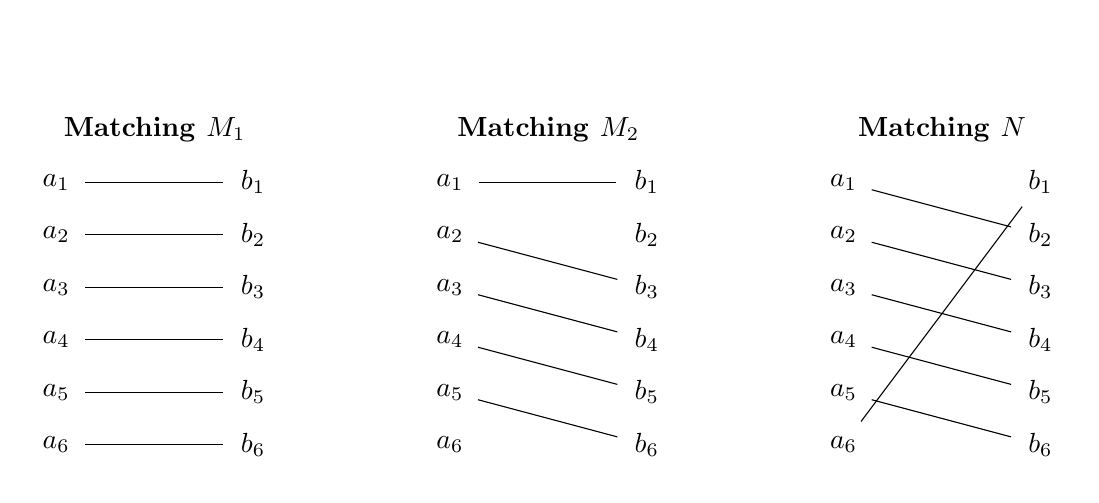
\begin{tikzpicture}[every node/.style={circle, draw=none}]
\node (A1) at (0,0/1.5) {$a_1$};
\node (A2) at (0,-1/1.5) {$a_2$};
\node (A3) at (0,-2/1.5) {$a_3$};
\node (A4) at (0,-3/1.5) {$a_4$};
\node (A5) at (0,-4/1.5) {$a_5$};
\node (A6) at (0,-5/1.5) {$a_6$};
\node (B1) at (2.5,0/1.5) {$b_1$};
\node (B2) at (2.5,-1/1.5) {$b_2$};
\node (B3) at (2.5,-2/1.5) {$b_3$};
\node (B4) at (2.5,-3/1.5) {$b_4$};
\node (B5) at (2.5,-4/1.5) {$b_5$};
\node (B6) at (2.5,-5/1.5) {$b_6$};

\node (AA1) at (5,0/1.5) {$a_1$};
\node (AA2) at (5,-1/1.5) {$a_2$};
\node (AA3) at (5,-2/1.5) {$a_3$};
\node (AA4) at (5,-3/1.5) {$a_4$};
\node (AA5) at (5,-4/1.5) {$a_5$};
\node (AA6) at (5,-5/1.5) {$a_6$};
\node (BB1) at (7.5,0/1.5) {$b_1$};
\node (BB2) at (7.5,-1/1.5) {$b_2$};
\node (BB3) at (7.5,-2/1.5) {$b_3$};
\node (BB4) at (7.5,-3/1.5) {$b_4$};
\node (BB5) at (7.5,-4/1.5) {$b_5$};
\node (BB6) at (7.5,-5/1.5) {$b_6$};

\node (AAA1) at (10,0/1.5) {$a_1$};
\node (AAA2) at (10,-1/1.5) {$a_2$};
\node (AAA3) at (10,-2/1.5) {$a_3$};
\node (AAA4) at (10,-3/1.5) {$a_4$};
\node (AAA5) at (10,-4/1.5) {$a_5$};
\node (AAA6) at (10,-5/1.5) {$a_6$};
\node (BBB1) at (12.5,0/1.5) {$b_1$};
\node (BBB2) at (12.5,-1/1.5) {$b_2$};
\node (BBB3) at (12.5,-2/1.5) {$b_3$};
\node (BBB4) at (12.5,-3/1.5) {$b_4$};
\node (BBB5) at (12.5,-4/1.5) {$b_5$};
\node (BBB6) at (12.5,-5/1.5) {$b_6$};

% Draw edges between the two sets of vertices
\draw (A1) -- (B1);
\draw (A2) -- (B2);
\draw (A3) -- (B3);
\draw (A4) -- (B4);
\draw (A5) -- (B5);
\draw (A6) -- (B6);

\node at (1.25,1/1.5) {\textbf{Matching }$M_1$};

\draw (AA1) -- (BB1);
\draw (AA2) -- (BB3);
\draw (AA3) -- (BB4);
\draw (AA4) -- (BB5);
\draw (AA5) -- (BB6);
% \draw (AA6) -- (BB1);

\node at (6.25,1/1.5) {\textbf{Matching }$M_2$};

\draw (AAA1) -- (BBB2);
\draw (AAA2) -- (BBB3);
\draw (AAA3) -- (BBB4);
\draw (AAA4) -- (BBB5);
\draw (AAA5) -- (BBB6);
\draw (AAA6) -- (BBB1);

\node at (11.25,1/1.5) {\textbf{Matching }$N$};

\end{tikzpicture}
\end{center}

$M$ is a stable matching since all $B$ vertices are matched and all vertices in $B$ except $b_1$ are in a tie and hence can't participate in a blocking pair. But $b_1$ is matched to its top choice and hence also cannot participate in a blocking pair. 

On transitioning from $M$ to $N$, all vertices in $A$ except $a_1$ are promoted and vertices $a_1$ and $b_1$ are both demoted. Hence we get a lower bound to popularity of $M$ as $u(M) \geq \frac{5}{2} = 2.5$ which is greater than the maximum tie length $k = 2$.

Now consider the matching $M_2$ of size 5. Since all vertices in $A$ except for $a_6$ are matched to their top choices, these cannot participate in a blocking pair. Also, all vertices in $a_6$'s preference list are matched to a vertex in their top tie. Hence, $M_2$ must be a stable matching. In fact, $M_2$ is also popular. To prove this consider another matching $M'$ and contest an election between $M_2$ and $M'$. The vertices $\{a_1, a_2, a_3, a_4, a_5, b_1, b_3, b_4, b_5, b_6\}$ are all matched to their top choice in $M_2$ and hence, $M'$ can never get these votes. Also, if $M'$ had the votes of $a_6$ or $b_2$ then it would lose the votes of $a_6$ and $b_2$'s matched partners in $M'$. Hence, $M'$ can never get more votes than $M_2$ and hence $M_2$ is popular and has popularity factor $1 \leq k = 2$

It is clear to see in this example that $M_1$ is the only matching of size 6 which is stable in the given instance and hence we have the following claim - 

\begin{theorem}
    There exists an instance such that no stable matching with size $> \frac{5}{6}|M_{opt}|$ has unpopularity factor $ \leq k$
\end{theorem}

\section{Future Work}
\begin{itemize}
    \item \textbf{Generalizing the $3 \times 3$ instance:} We have derived a characterization for instances that contain cycles in the popularity graph in the $3 \times 3$ case with strict and complete preference lists. One possible line of line of research is to work on such a generalization on the $4 \times 4$ case and then the general $n \times n$ case with strict complete preference lists. Once this is achieved, generalizing for the case of incomplete lists or ties in preferences could be another line of research.
    \item \textbf{Better size approximations with unpopularity guarantee:} In this report we discussed an algorithm formed by combining Kavitha's $k$ bounded unpopularity algorithm with Király's $\frac{2}{3}$ size approximation algorithm. An interesting line of research would be to combine Kavitha's bounded unpopularity algorithm with better size guarantee algorithms (such as Kavitha's $\frac{9}{13}$-size approximation algorithm) to obtain larger size stable matchings with bounded unpopularity.
    \item \textbf{Bounded unpopularity with two-sided ties:} A generalization of Kavitha's $k$ bounded unpopularity factor algorithm to the case with two-sided ties.
\end{itemize}

\section{Acknowledgements}
Firstly, I would like to thank Prof. Meghana Nasre for her continous guidance throughout the UGRC. 

I would also like to thank her PhD student Keshav Ranjan for guiding me on the vast literature related to the field. 

Lastly I thank Prof. N.S. Narayanaswamy for coordinating the UGRC.

\bibliographystyle{plain}
\bibliography{references.bib}

\end{document}
